\documentclass[answers]{exam}

% BASE TAKEN FROM ICCS315 SCRIBE NOTES

% --- SETUP STUFF ---
\usepackage[a4paper, margin=1in]{geometry}
\usepackage{enumitem}
\usepackage{booktabs}

\usepackage{url}
\usepackage[unicode]{hyperref}

\setcounter{secnumdepth}{2}

% --- MATH STUFF ---
\usepackage{amsthm, amsmath, amssymb}
\usepackage{mathtools,xspace}
\usepackage{nicefrac}

\usepackage{bbm}
\usepackage{dsfont}
\usepackage{cancel}

\usepackage{blkarray}
\newcommand{\matindex}[1]{\mbox{\scriptsize#1}} % Matrix index

% --- FONT STUFF ---
% Has to be under math stuff for some reason :/
\usepackage{newpxtext, newpxmath}
\usepackage[T1]{fontenc}

% --- DIAGRAM STUFF ---
\usepackage{tikz,pgfplots,xcolor,graphicx}
\usepackage{graphicx}
\usepackage{colortbl}
\usepackage{caption}
\usepackage{subcaption}

\usepackage[breakable,skins]{tcolorbox}
\usepackage{framed}
\usepackage{float}

\pgfplotsset{compat=1.18}

% --- THEOREM STUFF ---
\newtheorem{theorem}{Theorem}[section]
\newtheorem{proposition}[theorem]{Proposition}
\newtheorem{lemma}[theorem]{Lemma}
\newtheorem{corollary}[theorem]{Corollary}

\theoremstyle{definition}
\newtheorem{definition}[theorem]{Definition}
\newtheorem{example}[theorem]{Example}

\theoremstyle{remark}
\newtheorem{remark}[theorem]{Remark}
\newtheorem{claim}[theorem]{Claim}
\newtheorem{fact}[theorem]{Fact}

\usepackage{algorithm}
\usepackage[indLines=true]{algpseudocodex}
\usepackage{algorithmicx}
\algnewcommand\algorithmicinput{\textbf{Input:}}
\algnewcommand\Input{\item[\algorithmicinput]}
\algrenewcommand\algorithmicoutput{\textbf{Output:}}
\algrenewcommand\Output{\item[\algorithmicoutput]}
\algrenewcommand\algorithmicrequire{\textbf{Require:}}
\algrenewcommand\Require{\item[\algorithmicrequire]}

\renewcommand{\Pr}[1]{\mathbf{Pr}\left[#1\right]}
\newcommand{\CPr}[2]{\mathbf{Pr}\left[#1\ |\ #2\right]}
\newcommand{\Ex}[1]{\mathbf{E}\left[#1\right]}
\newcommand{\ExSub}[2]{\mathbf{E}_#2\left[#1\right]}
\newcommand{\CEx}[2]{\mathbf{E}\left[#1\ |\ #2\right]}

\newcommand{\Exp}[1]{\text{Exp}\left(#1\right)}
\newcommand{\Pois}[1]{\text{Poisson}\left(#1\right)}
\newcommand{\DGamma}[2]{\text{Gamma}\left(#1, #2\right)}
\DeclareMathOperator{\diam}{diam}

% === NOTES PORTION ===
% \begin{document}
%
% \frontmatter
% \thispagestyle{empty}

\begin{center}
\vspace{5cm}

\Huge{Graph Theory}

\vspace{5em}
\begin{center}
  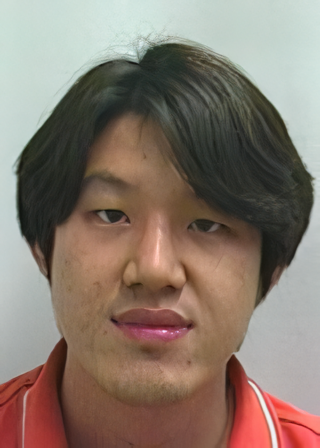
\includegraphics[height=0.5\textheight]{figures/chad.png}
\end{center}
\vspace{5em}

\Large Student's Notes for {T2/2023-2024}

\Large Written by {Nawat Ngerncham}

\Large Last updated: \today
\end{center}

%
% \setcounter{tocdepth}{1}
% \tableofcontents
%
% \mainmatter

% === HOMEWORK PORTION ===
\renewcommand{\questionlabel}{\textbf{Problem \thequestion.}}
\renewcommand{\solutiontitle}{}

\title{\Huge{{Homework 2}}
	\\
\Large\scshape{{Graph Theory and Combinatorics}}}
\author{{Nawat Ngerncham}}
\date{\today}

\begin{document}

\maketitle

\begin{questions}
  \setcounter{question}{3}
\question A graph \(G\) is \(k\)-critical if \(\chi(G)=k\) and if
  the deletion of any vertex yields a graph with smaller chromatic
  number.
  \begin{enumerate}[label=(\roman*)]
    \item Find all 2-critical and 3-critical graphs.
      \begin{solution} 
        Let us define the following term to help with this
        problem.

        \begin{definition}[Tree Portion]
          A \textit{tree portion} of a graph \(G\) is a
          subgraph \(T = G[\tau]\) where \(\tau\) is a set of
          vertices in \(G\) such that all but one vertex in
          \(\tau\) lies on a cycle and \(T\) is connected.
        \end{definition}
        
        \textbf{2-critical.} Claim that the only 2-critical graph
        is a tree of order 2.

        Indeed, we can remove either vertex and be left with
        one. In either case, we result in graph \(H\) such that
        \(\chi(H) = 1\).

        Note that all graphs \(G\) such that
        \(\chi(G) = 2\) are made up of the tree graph and cyclic
        graphs with even length where they are joined such that
        every cycle has even length. Otherwise, there is an odd
        cycle which requires 3 colors to color.

        \begin{center}
          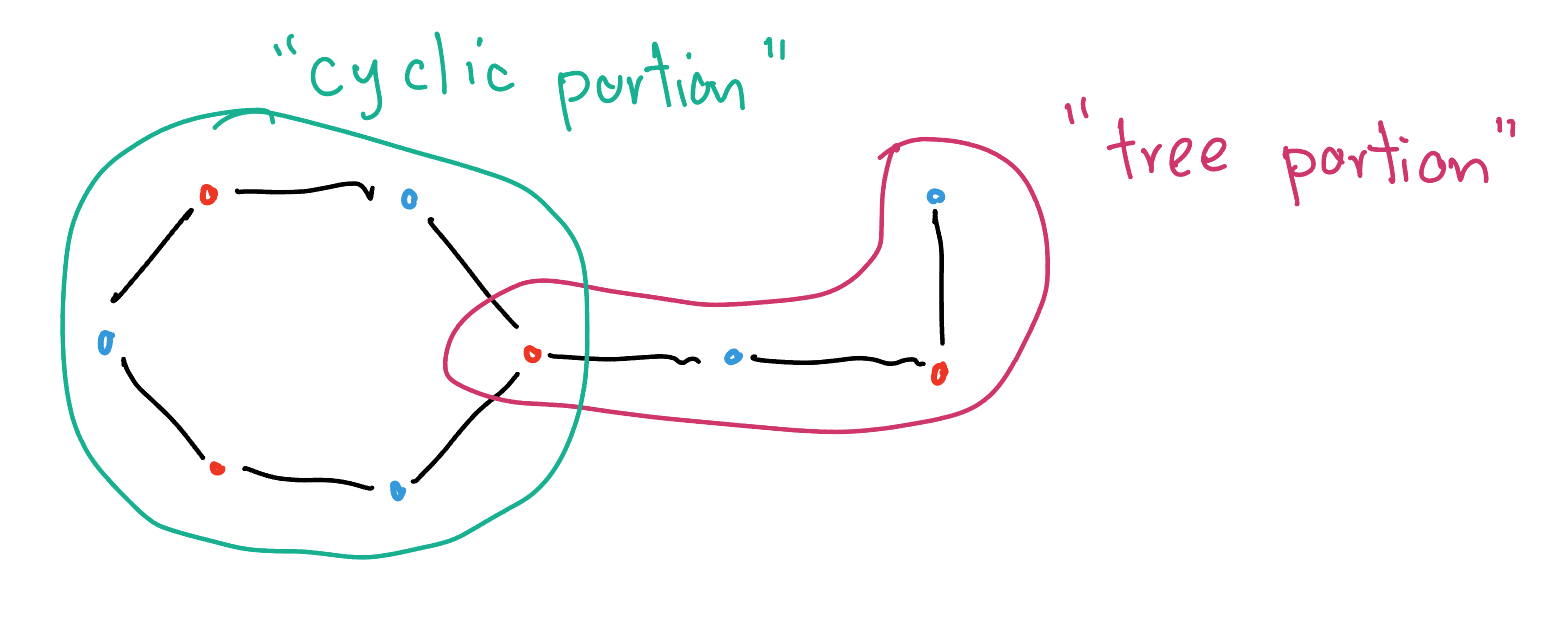
\includegraphics[width=0.6\textwidth]{figures/2-colorable}
        \end{center}

        Now, we will show that every other graphs with chromatic
        number 2 is not 2-critical. First, let \(T\) be any tree
        of order \(\geq3\). Recall the claim in part (iii) of this
        problem: If \(G\) is \(k\)-critical, then \(G\) has no
        cut-vertex. Since every vertex of \(T\) is a cut-vertex,
        \(T\) cannot be 2-critical by contrapositivity.

        Finally, let \(G\) be a graph with only even cycles. That
        is, every vertex \(v\) is part of an even cycle or is not
        in a cycle at all.
        \begin{enumerate}
          \item If \(v\) is not in any cycle, then \(v\) is in
            the \textit{tree portion} of \(G\). Consequently,
            \(v\) is either a cut-vertex or a leaf of the tree.
            If \(v\) is a leaf, then removing it does not change
            the chromatic number. If \(v\) is a cut-vertex, then
            \(G\) is not 2-critical by the result below. In both
            cases, \(\chi(G - v)\) does not change from
            \(\chi(G)\).

          \item Otherwise, \(v\) is part of an even cycle, say
            \(C\). Note that \(v\) can be part of multiple cycles
            but we can just apply this argument on every cycle
            \(v\) is a part of. Observe that \(C - v\) is a tree.
            Then, by the same argument as above, \(C-v\) has the
            same chromatic number and consequently, so does
            \(G\).
        \end{enumerate}
        Therefore, the tree of order 2 is the only 2-critical
        graph.

        \vspace{5em} 

        \textbf{3-critical.} Claim that a graph is 3-critical
        if and only if \(G = C_n\) for some odd \(n\).

        We will first the reverse direction since it is simpler.
        Let \(G\) be a cyclic graph of odd length \(n\). Hence,
        \(\chi(G) = 3\). Removing any vertex in \(G\) results in
        a tree. Thus, \(\chi(G-v) = 2\) for any \(v \in V(G)\).
        Therefore, \(C_n\) with \(n\) odd is 3-critical.

        We will now show the forward direction. Let \(G\) be a
        3-critical graph. Then, \(G\) must contain an odd cycle,
        say \(C\). Suppose to contradict that \(G\) contains 
        at least one of the following:
        \begin{itemize}
          \item an even cycle,
          \item a \textit{tree portion}; or
          \item another odd cycle \(C' \neq C\). 
        \end{itemize}
        Observe that removing any vertex from the above subgraphs
        does not disconnect \(C\). So, \(\chi(G-v)=3\) for any
        \(v\) in an even cycle, a tree portion, or another distinct
        odd cycle subgraph of \(G\). Therefore, every 3-critical
        graph cannot contain an even cycle, a tree portion, and
        can only have one unique odd cycle. Therefore, a
        3-critical graph is a \(C_n\) with \(n\) odd.
      \end{solution}

    \item Give an example of a 4-critical graph,
      \begin{solution}
        \centering
        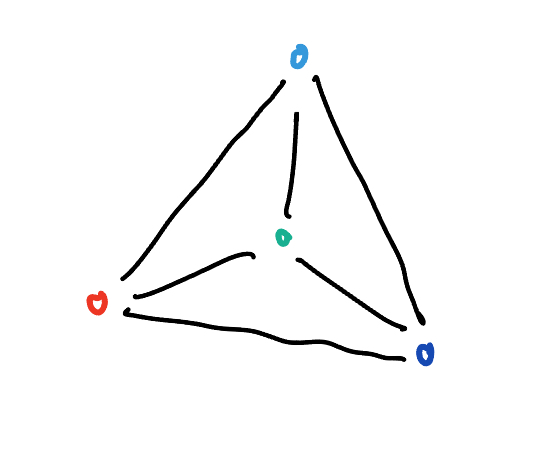
\includegraphics[width=0.3\textwidth]{figures/4-critical}
      \end{solution}

    \item Prove that, if \(G\) is \(k\)-critical, then
      \begin{enumerate}[label=(\alph*)]
        \item every vertex of \(G\) has degree at least \(k-1\),
          \begin{solution}
            Suppose to contradict that there exists a vertex
            \(v\) such that \(\deg v < k-1\). Note that \(G-v\)
            is \((k-1)\)-colorable since \(G\) is \(k\)-critical.
            Note also that there must be a color \(c\) in the
            \((k-1)\)-coloring such that \(v\) is not adjacent to
            any vertex colored with \(c\) since there are \(k-1\)
            colors but \(v\) is adjacent to less than that many
            vertices. This is a contradiction since we can then
            color \(v\) with \(c\) since it is not adjacent to
            any vertex colored with \(c\) but \(G\) would still
            be \((k-1)\)-colorable. Therefore, a \(k\)-critical
            graph \(G\) satisfies \(\delta(G) \geq k-1\).
          \end{solution}

        \item \(G\) has no cut-vertices.
          \begin{solution}
            We will show this using contrapositivity: Let \(G\)
            be a \(k\)-chromatic graph with a cut-vertex \(x\).
            We will show that \(G\) is not \(k\)-critical.

            Suppose that \(G-v\) is split into components
            \(G_1, G_2, \ldots, G_c\) where \(c\) is the number
            of components. Abusing notation, let \(G_i \cup
            x\) be the \textbf{induced subgraph} of \(V(G_i)
            \cup x\). Observe that 
            \[
              \chi(G) =
              \max_{i \in 1..c} \chi(G_i \cup x)
            \]
            This is because every induced subgraph \(G_i \cup x\)
            is disjoint except at \(x\). So, we can color them
            independently after assigning a color for \(x\) and
            the chromatic number of \(G\) is the same as the
            component with the highest chromatic number.

            Let \(G_j \cup x\) be a component with the highest
            chromatic number. That is, 
            \[
              \chi(G_j \cup x) = \max_{i \in 1..c} \chi(G_i \cup x) 
            \]
            Note that \(G_j\) may not be unique. Still, removing
            any vertex \(v\) from any component other than \(G_j\)
            would not change the chromatic number of \(G-v\).
            That is, \(\chi(G) = \chi(G-v)\). Thus, \(G\) is not
            \(k\)-critical.
          \end{solution}
      \end{enumerate}
  \end{enumerate}

  \question A connected bipartite graph \(G\) has partite sets 
\(U\) and \(W\), where \(|U| = |W| = \) \(k \geq 2\). Prove that
if every two vertices of \(U\) have distinct degrees in \(G\),
then \(G\) contains a perfect matching.

\begin{solution}
  
\end{solution}

  \begin{hwproblem}{3}{
    Give two examples of non-isomorphic 3-regular graphs of order 10.
  }
  From the figure below, we can see that the two graphs are not isomorphic 
  since we can identify a cycle of length 3 in the left graph but not in the 
  right graph. Thus, they are non-isomorphic.
  \begin{center}
    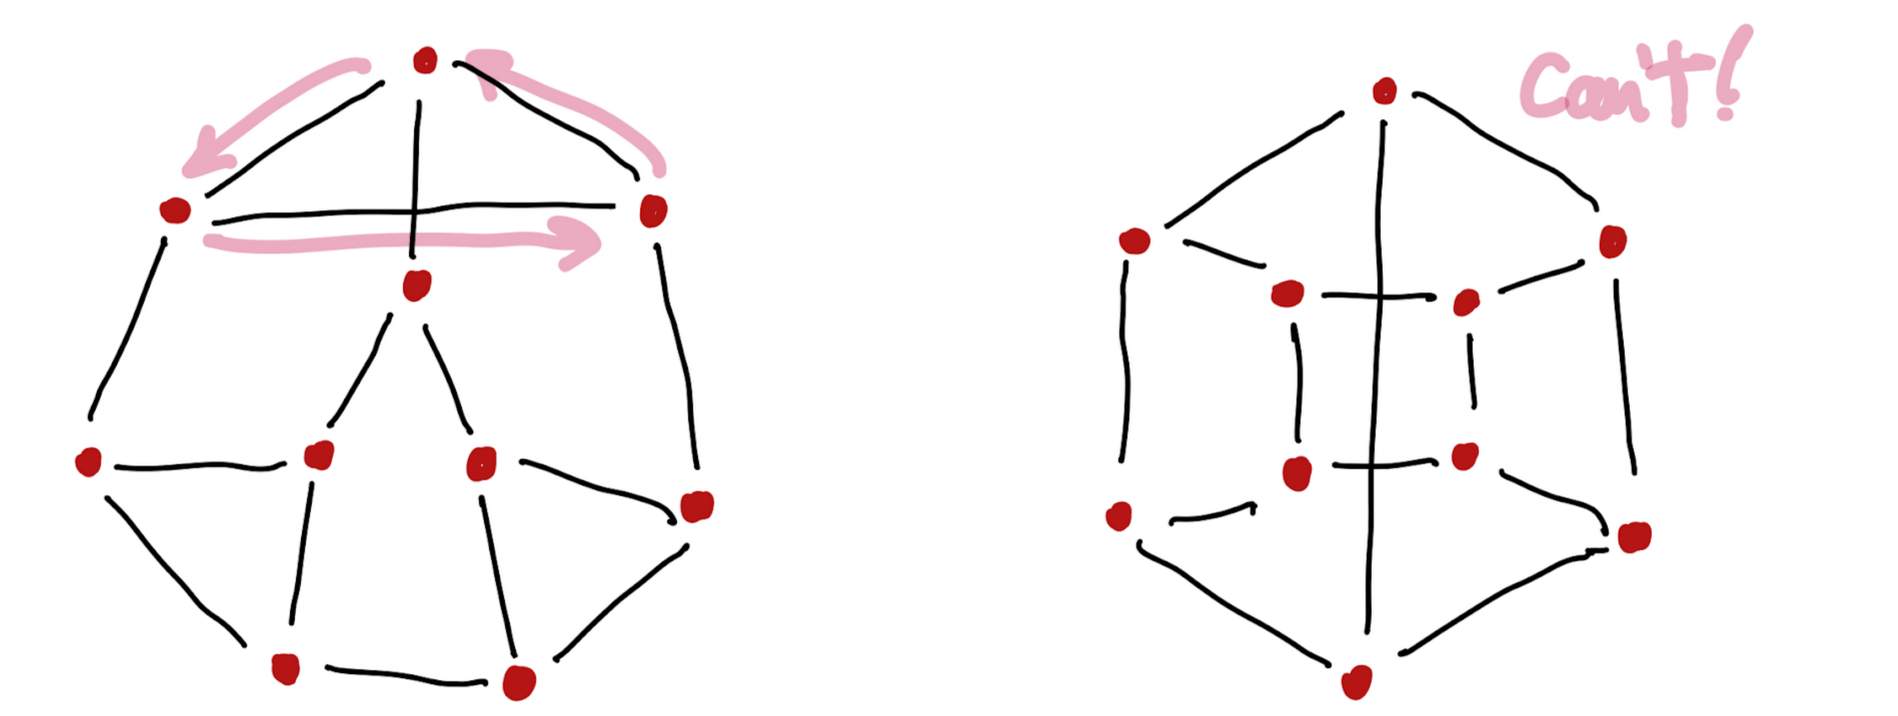
\includegraphics[width=0.69\textwidth]{figures/p3}
  \end{center}
\end{hwproblem}

  \question Derive K\"onig's Theorem from the \textit{Max-flow,
min-cut} theorem.

\begin{solution}
  
\end{solution}

  \question Let \(G\) be connected graph of order \(n\) where
\(\Delta(G)+\delta(G) \geq n-2\). Show that \(\operatorname{diam}
(G) \leq 4\).

\begin{solution}
  We will show that for every pair of distinct vertices \(u, v\),
  \(d(u, v) \leq 4\). Let \(x\) be the vertex of maximum degree.
  We will show the different cases possible for which 
  neighborhood \(u, v\) belongs to. Note that we will consider
  these cases without loss of generality and assume that \(u\) is
  the start of the path \(u \to v\).

  \begin{enumerate}[label=\Roman*.]
    \item If \(u \in N(v)\), then they are adjacent and
      \(d(u, v) = 1\).
    \item If 
  \end{enumerate}
  % Claim that for every \(v \in V(G)\), we have that \(d(v, x)
  % \leq 2\). If this satisfies, then we can always route any two
  % vertices through \(x\), achieving distances of at most
  % \(2+2=4\).
  % If \(v \in N(x)\), then we are done and \(d(v, x) = 1\).

  % Otherwise, we would have that \(v \notin N(x)\).
  % % Notice that \(\deg v + \deg x < n\).
  % For simplicity's sake, we say that any vertex is adjacent to
  % itself even though there is no edge to itself. 
  % Recall that \(\deg x = \Delta\). Then, there are \(n - (\Delta
  % + 1)\) vertices not adjacent to \(x\) where \(\Delta\) is every
  % neighbor of \(x\) and 1 is \(x\) itself. Consider the
  % following. Since \(\Delta + \delta \geq n-2\), it follows that
  % \(\Delta \geq n - \delta - 2\). Then, the number of vertices
  % not adjacent to \(x\) is
  \[
  \begin{aligned}
    % n - (\Delta + 1) 
    %   &\geq n - (n - \delta - 2 + 1) \\
    %   &= \delta + 1
    \delta \geq n - \Delta - 2
  \end{aligned}
  \]

  Therefore, we can conclude that for any connected graph \(G\)
  of order \(n\) where \(\Delta(G) + \delta(G) \geq n-2\),
  \(\diam(G) \leq 4\) satisfies. 
\end{solution}

  \question
  Write the programs to perform a bijective mapping between the labelled trees and Prüfer's codes.
  \begin{parts}
    \part
      Input: labelled tree $H$ (Use any data structure for the tree as you like)
      Output: Prüfer's codes that corresponding to $H$.
    \part
      Input: Prüfer's codes
      Output: labelled tree $H$ that corresponding to the code.
    \part
      Input: number of vertices $n, n \geq 3$
      Output: the set of all Prüfer's codes of length $n-2$ and its corresponding
      labelled tree of $n$ vertices.
  \end{parts}
  Verify by hand for $n=3,4$ that Program \#3 is indeed a bijective map.

\end{questions}

% in case of needing citations
\bibliographystyle{plainurl}
\bibliography{refs}

\end{document}
